\documentclass[a4paper, 11pt]{article}

\usepackage[utf8]{inputenc}
\usepackage[T1]{fontenc}
\usepackage[francais]{babel} 
\usepackage{amsmath} % pour les formules de maths
\usepackage{amssymb} % pour des symboles
\usepackage{mathrsfs} % pour avoir acces a des jolies lettres calligrafiées. :)
\usepackage{listings} % pour le code source
\usepackage{color} % pour les couleurs
\usepackage{graphicx} % pour les graphiques (images)
\usepackage{fancyhdr} % pour utiliser le pagestyle fancy
\usepackage[headheight=14pt]{geometry} % pour les marges

\geometry{hmargin=3cm}

\title{\textbf{Métaheuristique pour l'optimisation}\\Série 2: The Quadratic assignment problem}
\author{Romain Mencattini}
\date{\today}

\pagestyle{fancy} % pour avoir des entetes et des pieds de page
\renewcommand\headrulewidth{0.6pt}
\fancyhead[L]{Romain Mencattini} % haut de page gauche
\fancyhead[R]{Université de Genève \today} % haut de page droite

\begin{document}
\maketitle
\newpage
\tableofcontents
\newpage

\section{Quadratic Assignment Problem}
\paragraph{}
Nous allons expliquer le problème afin de bien saisir les enjeux du problème.
Les problèmes d'assignation quadratiques sont une famille de problèmes qui demandent d'assigner des objets ou \textit{facilities} à 
une place ou \textit{locations}.
On peut imaginer un exemple, (repris dans l'énoncé du tp) où les objets sont des usines et les places des villes. On souhaite placer au
mieux les usines dans les dites villes.

Le critère de qualité est une fonction $F$ qui est définie comme suit:
\begin{center}
 $arg \ \min\limits_{\psi \in S(n)} \ I(\psi) = \sum\limits_{i,j=1,...,n} w_{ij} \cdot d_{\psi_i,\psi_j}$
\end{center}

Où $w_{ij}$ correspond au flux entre l'objet $i$ et l'objet $j$, et $d_{\psi_i,\psi_j}$ correspond à la distance entre la place de 
l'objet $i$ et la place de l'objet $j$.

Ces éléments sont donnés par deux matrices. La matrice $W$ et la matrice $D$ qui sont de tailles $n\ $x$\ n$. Avec $n$ qui est la taille de 
notre solution. Les matrices $W,D$ sont symétriques et leur diagonale est nulle.

Le but est de trouver un vecteur de taille $n$ qui à chaque place fait correspondre un objet de manière que la fonction $F$ soit minimale.

\section{Tabu Search}
\paragraph{}Expliquons maintenant la recherche tabou ainsi que ses subtilités.
La recherche se déroule comme suit:

\subsection{Génération d'une solution}
\paragraph{}On génère une solution aléatoire. La solution sera de taille $n$. Avec les $n$ objets placés de manière aléatoire sur les $n$
places du vecteur solution.
On pose que $best = F(solution)$. Car on désire garder en mémoire le meilleur résultat rencontré.

\subsection{Génération de voisins}
\paragraph{}
Pour une solution donnée, soit $x_0$. On veut calculer $V(x_0)$.
Pour ce faire, on définit que les voisins de $x_0$, qui sont tous les solutions égalent à $x_0$ à une permutation près.
Donc:
\begin{center}
  $x_0 = (1,2,3,4)$\\
  $x_1 = (2,1,3,4) \in V(x_0)$
\end{center}

Une fois ces voisins générés, on va les trier selon leur fitness. On applique donc $F(x_i)$, où $x_i \in V(x_0)$. Et on trie selon
ce critère.

\subsection{Choix du voisins}
\paragraph{}
Le choix du voisins se fait de la manière suivante:
\begin{enumerate}
 \item Si $F(x_i) < F($best$)$, alors on choisit $x_i$, où $x_i$ est notre meilleur voisin
 \item Si la condition 1. n'a pas fonctionné, on prend le meilleur voisin non tabou.
\end{enumerate}

Une fois ce choix fait, on met à jour $best$.

\subsection{Liste Tabou}
\paragraph{}
Dans le cas de ce programme, on a implémenté la liste tabou comme étant une matrice de taille $n$ x $n$.
Après l'échange de l'objet $i$ en position $r$ avec $j$ en position $s$, on va interdire l'échange inverse, soit l'objet $i$ en position 
$s$ et l'objet $j$ en position $r$.
Pour ce faire, dans la matrice, à l'indice $(i,s)$, on va inscrire $t+l$, où $t$ est la valeur de l'itération courante et $l$ une valeur
fixée. Même chose pour $(j,r)$.
On interdit donc le fait, si $t' < t+l$ de faire l'échange inverse en regardant dans les cases $(i,s)$ et $(j,r)$.

\subsection{Calcule de Fitness}
\paragraph{}
Une astuce pour ne pas devoir calculer la fitness à chaque fois, qui est en $O(n^2)$. On va simplement calculer la différence qui est, 
elle, en $O(n)$. On peut faire cela car il y a beaucoup d'éléments qui ne dépendent pas d'$i$ et $j$. Voici donc la formule:
\begin{center}
 $\Delta(\psi_i,\psi_j) = 2 \cdot \sum\limits_{k \ne i,j}(w_{j,k}-w_{i,k}(d_{\psi_i,\psi_k} - d_{\psi_j,\psi_k})$
\end{center}
On a une simple somme, donc le gain calculatoire est conséquent par rapport à une double somme.

\section{Résultats}
Afin d'avoir une représentation, nous avons dessiné les valeurs de fitness ainsi que le meilleur résultat. Cela permet de voir l'impacte
de $l$ sur la recherche.

Pour $l=1$:
\\
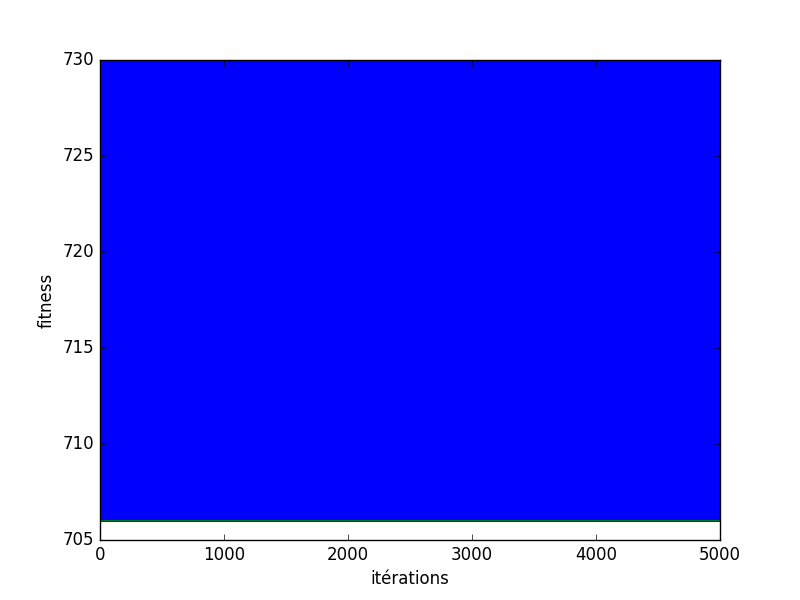
\includegraphics[scale=0.5]{l_1}
\\
On voit dans ce cas là, que l'algorithme ne prend que deux valeurs de fitness et fait des aller-retour entre.
Cela vient du fait, que la taille de la liste tabou vaut 1. Donc il visite une autre valeur, et ensuite il peut revenir sur l'ancienne.
Il tombe donc dans le premier minimum local et n'en sort plus.
On va voir qu'il est possible de corriger cela en modifiant la valeur de $l$.

Pour $l=0.5n$:
\\
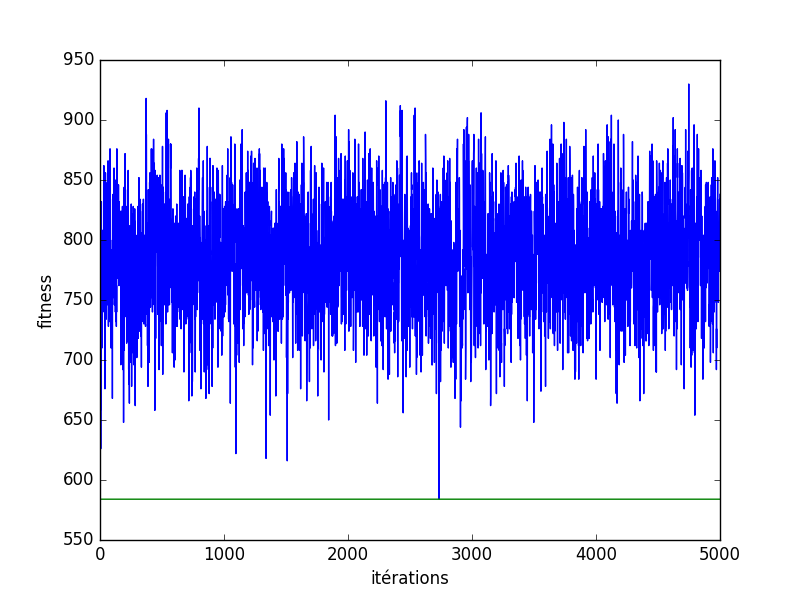
\includegraphics[scale=0.5]{l_0_5}
\\
Cette fois ci, malgré qu'il tombe dans certain minima local. La taille de la liste, lui permet d'en sortir pour aller voir autre part dans
l'espace de recherche.
On remarque également que les fitness varient beaucoup et rapidement. C'est donc une indication sur la difficulté du problème.

Pour $l=0.9n$:
\\
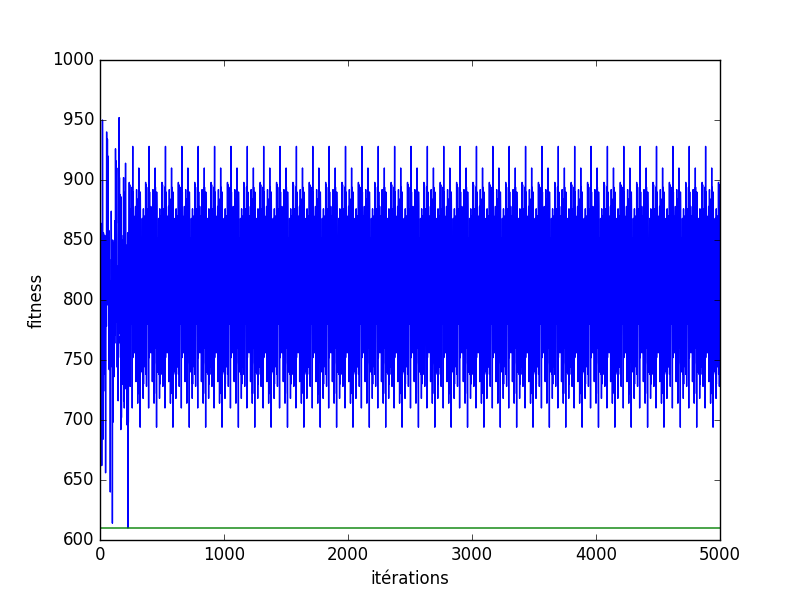
\includegraphics[scale=0.5]{l_0_9}
\\
Ici, l'algorithme va trouver un minimum local, puis va continuer d'explorer l'espace de recherche pour trouver le minimum global (dans
cette configuration et pour ce nombre d'itération). Puis il va partir dans une boucle avec un pattern visible.
\paragraph{}
Les résultats me paraissant étonnants, j'ai généré un nouveau problème de taille $n=12$, de manière aléatoire et j'ai relancé mon algorithme
pour avoir un deuxième graphique:
\\
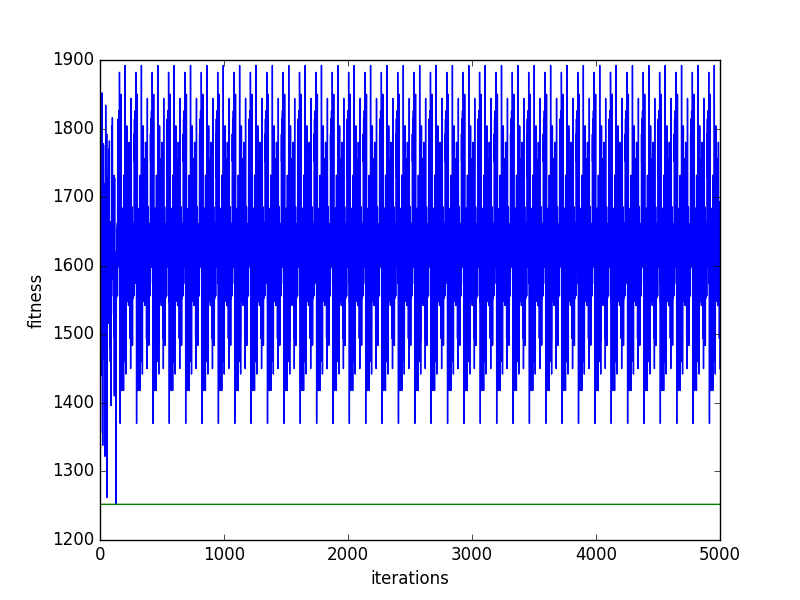
\includegraphics[scale=0.5]{l_0_9_a}
\\
On voit le même genre de résultat.

\paragraph{}
Voici les résultats demandés sur dix lancés d'algorithme:
\\
\begin{tabular}{|l|c|c|c|}
\hline
1.dat & best & moyenne & déviation standard\\
\hline
l= 1 & 626.0 &731.28812	& 39.2576559013 \\
\hline
l= 0.5n& 544.0 & 788.65092 & 43.031624454\\
\hline
l= 0.9n	&558.0	& 811.55036 & 55.8561665698 \\
 \hline
\end{tabular} 
\\
\paragraph{}
On remarque que pour $l=1$, le fait de tomber dans un minimum local diminue grandement la déviation standard. Car il n'y a que deux 
valeurs différentes.
Pour $l=0.5n$, il y a une grande différence entre le meilleur et la moyenne. Cela vient du fait que l'exploration continue même une fois 
qu'un minimum local est trouvé.
Même chose pour $l=0.9n$, sauf que la différence est énorme, du à la boucle qui se crée dans l'exploration.

\paragraph{}
\begin{tabular}{|l|c|c|c|}
\hline
 & best & moyenne & déviation standard\\
\hline
40.dat & & & \\
\hline
l= 0.5n &18440.0 &19598.156 &295.173982024\\
\hline
 & & & \\
 \hline
50.dat & & & \\
\hline
l= 0.5n &29958.0 & 31371.912 & 334.404557768\\
\hline
 & & & \\
 \hline
80.dat & & & \\
\hline
l= 0.5n & 78396.0 & 80086.626 & 533.669916825\\
\hline
 & & & \\
100.dat & & & \\
\hline
l= 0.5n & 122550.0 & 124811.564 & 828.609559385\\

\hline
\end{tabular}
\paragraph{}
Outre le fait que les valeurs deviennent extrêmement grande, on retrouve le même genre de résultat que pour $1.dat$. Cela est donc
cohérent entre les données.

Un point est à soulever: les performances. Ayant écrit le programme en Python, lorsque $n$ devient grand (pour $n=40,50,80,100$).
Le temps de calcul devient bien trop important. Nous avons tenté de regarder si des optimisations étaient possibles en nous basant sur des
outils de \textit{profiling} tel que:
\begin{itemize}
 \item CPython: pour savoir dans quelle fonction notre programme passait le plus de temps. La réponse est la fonction $delta$.
 \item Line Profiler: pour savoir combien de temps passer notre programme dans une fonction et quelles lignes demandent plus de calculs
 que d'autres. Il s'agit de la boucle de calcule du $\Delta$
\end{itemize}
Malgré cela, il ne nous a pas été possible d'optimiser notre programme. Cependant heureusement qu'on a utilisé le $\Delta$ en $O(n)$ et 
non la fitness en $O(n^2)$.
Dans le cadre d'un travail pratique universitaire pour comprendre un algorithme cela peut suffire. 
Cependant en vue de résoudre un problème concret, il nous faudra un langage plus adapté et avec de meilleures performances.


\end{document}


